%--------------------------------------------------
% IR Tracking Documentation
%--------------------------------------------------
\documentclass[letterpaper,11pt]{article}

%--------------------------------------------------
% Declaration section
%--------------------------------------------------
\usepackage{graphicx}
\usepackage{subfigure}
\usepackage[pdfauthor={GuyGuy}, pdftitle={Survival Records Documentation}, pdfsubject={Software Manual}, pdflang={English}]{hyperref}
\usepackage{amsmath}
\usepackage{amssymb}
\usepackage{listings}
\usepackage{textcomp}
\usepackage{color}
\usepackage[usenames,dvipsnames]{xcolor}
\usepackage[margin=1in]{geometry}
\usepackage{ccaption}
\usepackage{times}
\usepackage{fancyhdr}
\usepackage{lastpage}
\usepackage{url}
\usepackage{breakurl}
%\usepackage{mnsymbol}
\usepackage{tikz}

\hypersetup{linktocpage=true,colorlinks=false,linkcolor=blue,citecolor=blue,pdfpagemode=UseNone,pdfstartview={XYZ 1000 1000 1}}

% Change the format of a figure caption
% For more options see the package documentation
\captionnamefont{\bfseries}
\captiontitlefont{\small}
\captiondelim{ --- }
\hangcaption
\renewcommand{\figurename}{Figure}

\renewcommand{\thesubfigure}{\thefigure.\arabic{subfigure}}
\makeatletter
\renewcommand{\p@subfigure}{}
\renewcommand{\@thesubfigure}{\thesubfigure:\hskip\subfiglabelskip}
\makeatother

\hypersetup{linktocpage=true,colorlinks=false,linkcolor=blue,citecolor=blue,pdfpagemode=UseNone,pdfstartview={XYZ 1000 1000 1}}

\definecolor{dkgreen}{rgb}{0,0.6,0}
\definecolor{gray}{rgb}{0.5,0.5,0.5}
\definecolor{mauve}{rgb}{0.58,0,0.82}
 
\lstset{ %
  basicstyle=\ttfamily \footnotesize,           % the size of the fonts that are used for the code
  numbers=left,                   % where to put the line-numbers
  numberstyle=\tiny\color{gray},  % the style that is used for the line-numbers
  stepnumber=1,                   % the step between two line-numbers. If it's 1, each line 
                                  % will be numbered
  numbersep=5pt,                  % how far the line-numbers are from the code
  backgroundcolor=\color{white},      % choose the background color. You must add \usepackage{color}
  showspaces=false,               % show spaces adding particular underscores
  showstringspaces=false,         % underline spaces within strings
  showtabs=false,                 % show tabs within strings adding particular underscores
  frame=single,                   % adds a frame around the code
  rulecolor=\color{black},        % if not set, the frame-color may be changed on line-breaks within not-black text (e.g. commens (green here))
  tabsize=2,                      % sets default tabsize to 2 spaces
  captionpos=b,                   % sets the caption-position to bottom
  breaklines=true,                % sets automatic line breaking
  breakatwhitespace=false,        % sets if automatic breaks should only happen at whitespace
  title=\lstname,                   % show the filename of files included with \lstinputlisting;
                                  % also try caption instead of title
  keywordstyle=\color{blue},          % keyword style
  commentstyle=\color{dkgreen},       % comment style
  stringstyle=\color{mauve},         % string literal style
  escapeinside={\%*}{*)},            % if you want to add a comment within your code
  morekeywords={*,...}               % if you want to add more keywords to the set
}

%--------------------------------------------------
% Headings
%--------------------------------------------------
\fancypagestyle{plain}{
\fancyhead{} % clear all header fields
\fancyhead[LO,RE]{\normalsize \slshape Survival Records Documentation}
\fancyhead[RO,LE]{\normalsize \slshape \leftmark}

\fancyfoot{} % clear all footer fields
\fancyfoot[LE,RO]{\normalsize \thepage\ of \pageref*{LastPage}} % insert page numbers
\renewcommand{\headrulewidth}{0.7pt}
\renewcommand{\footrulewidth}{0.7pt}
}

\renewcommand{\sectionmark}[1]{\markboth{\thesection.\ #1}}

\setcounter{tocdepth}{2}

%--------------------------------------------------
% Document Environment
%--------------------------------------------------
\begin{document}

\pagenumbering{roman}
\begin{titlepage}
\begin{flushright}
\footnotesize
Written by: \texttt{guyguy}
\today
\end{flushright}

\vspace*{\fill}
\begin{center}
\begin{tikzpicture}
	\draw (0, 0) node[align=center, inner sep=0] {
\includegraphics[width=\columnwidth]{cover}};
	\draw (0, 1) node[align=center] {\textsc{\huge \color{White} Survival Records Documentation}};
\end{tikzpicture}
\end{center}
\tableofcontents
\vspace*{\fill}
\end{titlepage}
\newpage

%\listoftables
%\listoffigures
%\newpage

\pagenumbering{arabic}
\pagestyle{plain}
\section{Introduction}
This document shows how to use the survival records script for setting up automatically updated survival records that are displayed on Google Spreadsheets.
\paragraph{Small note}
I am going to try to update this document with a lot of screenshots to make it an easy step-by-step tutorial. However, the spreasheet is constantly being changed so the actual document may end up looking different.
\subsection{Purpose}
Why should we bother with keeping track of survival records anyway? This project is not as serious as it seems and mostly serves as a sideproject of mine. It serves as a way for me to learn Python and to practice a little bit of programming. Other than that, the records are not meant to be taken very seriously. However, it is good to keep track of and recognize achievements made by our community of survival players.

There are many people playing survival mode in Left 4 Dead 1 and Left 4 Dead 2 from all over the world, and it is a good opportunity to make new online friends and collaborate with them towards a common goal. The Left 4 Dead series are known to be high quality cooperative games that stress teamwork, and the addition of goals and records makes the game refreshing and endlessly replayable for many survival enthusiasts.

\subsection{How it works}
After each game of survival, the game displays the statistics of the round that you just played. This includes the duration of the round and the number of common infected, special infected and tanks killed. The numbers will typed by someone (maybe you!) onto a Google Spreadsheet for the purpose of keeping track of records. Once the numbers are input onto the spreadsheet, the spreadsheet maintainer runs the provided Python script in order to update the spreadsheet. The best time, kills, and other statistics are calculated and displayed on the updated spreadsheet. In the next sections, the software behind the recording system will be explained.

\subsubsection{Google Spreadsheets}
Google spreadsheets is part of the Google Docs office suite, which is an online service designed to allow users to collaborate on office documents. The spreadsheets are a collection of tables, and consist of multiple pages called worksheets. \figurename\ \ref{fig:sample1} shows what a Google Spreadsheet looks like in a web browser.
\begin{figure}[htb!]
\centering
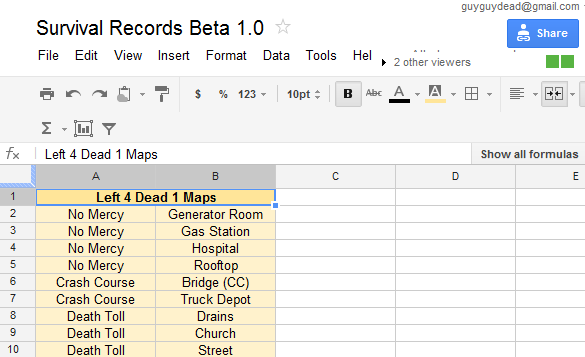
\includegraphics[width=0.40\columnwidth]{sample_screen_1}
\caption{Google Spreadsheet Opened in Web Browser}
\label{fig:sample1}
\end{figure}

One of the interesting features of Google Docs is that any changes made to the web documents are instantly updated and seen by people on the Internet. In this way, we can imagine having a document that outputs real-time statistics, in our case, of the game Left 4 Dead.

\subsubsection{Google Data API}
As well as being able to edit spreadsheets from a web browser, Google has provided a way to communicate to their servers and automatically update Google Spreadsheets: the Google Data API (Application Programming Interface). What this means is that anyone can download the provided programming library and use it to read from and write to a Google Spreadsheet by writing a simple program.

\subsubsection{Python}
Python is a relatively new programming language suitable for scripting. I chose Python because it is an interesting language that I wanted to learn through this project. \figurename\ \ref{fig:sample2} shows the output of a sample run of the Python script to update the Google Spreadsheet.
\begin{figure}[htb!]
\centering
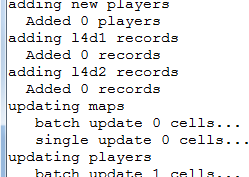
\includegraphics[width=0.30\columnwidth]{sample_screen_2}
\caption{Python Script Updating the Spreadsheet}
\label{fig:sample2}
\end{figure}

\section{Spreadsheet Overview}
This section will explain how the Google Spreadsheet works without going into the details of the underlying script. This section is for users that want to look at the survival records through the web browser and are not necessarily concerned with how it is updated. The spreadsheet is divided up into a number of different worksheets. Each worksheet will be explained in the following sections. The steps to adding records to the spreadsheets will be explained in Section \ref{sec:adding}.

\subsection{Maps}
The worksheet titled maps displays the list of official survival maps in Left 4 Dead 1 and 2 (see \figurename\ \ref{fig:sample_maps}). The first column indicates the campaign and the second column indicates the map. The names used here should be used in the rest of the document. For example, refer to the map as ``Street'' as shown and not other variations such as ``The Street''.

\subsection{Players}
This worksheet displays a list of survival players (see \figurename\ \ref{fig:sample_players}). Note that firstly, this is definitely not a complete list of all the players, only the players that are registered in the system. Secondly, the names of some players have been modified for readability. Their full name might appear under the aliases column. When referring to a player, you can use either the player's name or one of his aliases.

The country where the player is located is only a guess based on looking at public steam profiles, and might not actually be accurate. In the cases where I didn't know where the player was located, his country is listed as ``Unknown''.

\subsection{Records}
This worksheet (\figurename\ \ref{fig:sample_records}) displays the lists of all records in the system. These are the master lists of all records, not just best time, best kills, and also there are no exceptions or special groupings considered.

\paragraph{Dates}
Since the date is not an important factor in the survival statistics, not all the dates may be accurate. Firstly, the dates recorded consider the North American central timezone. Secondly, when the actual date that the survival game took place could not be found due to lack of screenshots, I made up an approximate date.

\begin{figure}[htb!]
\centering
\subfigure[Maps Worksheet] {
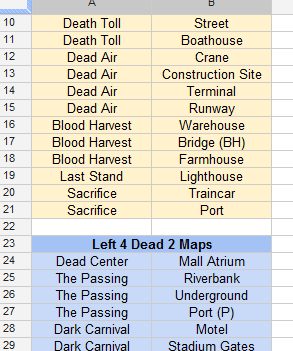
\includegraphics[width=0.30\columnwidth]{sample_maps}
\label{fig:sample_maps}
}
\subfigure[Players Worksheet] {
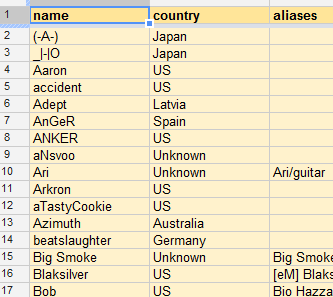
\includegraphics[width=0.30\columnwidth]{sample_players}
\label{fig:sample_players}
}
\subfigure[Records Worksheet] {
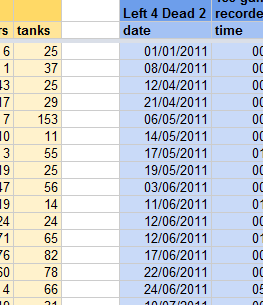
\includegraphics[width=0.30\columnwidth]{sample_records}
\label{fig:sample_records}
}
\caption{Examples of the Worksheets}
\end{figure}

\subsection{Statistics}
This worksheet is where all the major statistics are calculated. It consists of a number of tables for Left 4 Dead 1 and 2, which are mostly self-explanatory. The tables show the best record in the system for all of the official Left 4 Dead 1 and 2 maps. I will now explain all the possible statistics that are tracked.

\subsubsection{Time}
This statistic measures the time the round has lasted. It is traditionally how all survival games have been rated.

\subsubsection{Trash Factor}
This statistic was named the trash factor or trash4cash factor after the player who first started mentioning this statistic to be used for measuring the difficulty of survival games. It is the ratio of total SI kills to minutes played. Specifically,
\begin{align}
TF_{1} &= \frac{smokers + boomers + hunters}{minutes} \\
TF_{2} &= \frac{smokers + boomers + hunters + chargers + spitters + jockeys}{minutes} \text{.}
\end{align}

This factor is meant to be interpreted as a difficulty rating of 1-10, where 10 is a most difficult round due to high number of special infected. In actuality, the trash factor may also exceed 10, but this seems to happen rarely, during survival rounds that should be considered difficult.

\subsubsection{Kill Factor}
This statistic takes the average kills of each kind of special infected including tanks. The reasoning for this is to penalize rounds that have a small number of a specific kind of special infected due to them getting stuck. For example, if all jockeys are stuck at some point, the number of special infected may still be significant, but the difficulty in dealing with jockeys are removed and the survival round was overall less challenging. Kill factor is calculated as follows:
\begin{align}
KF_{1} &= \frac{(smokers + boomers + hunters + tanks) / 4}{minutes} \\
KF_{2} &= \frac{(smokers + boomers + hunters + chargers + spitters + jockeys + tanks) / 7}{minutes} \text{.}
\end{align}

This factor should yield values around 1.0. Factors well below 1.0 should be considered easy rounds and factors well above 1.0 should be considered difficult rounds.

\subsubsection{Other Factors}
Other factors include tank factor, gore factor, and common factor. These are pretty self-explanatory; tank factor is the total tank kills, common factor is the total common kills, and gore factors is the total amount of SI kills.

\subsection{Top 10}
This shows the same statistics as before, except the best 10 times are recorded for each map.

\subsection{NA Statistics}
These statistics are the same as the previous section's statistics, except that it only includes records with over 50\% of the players residing in North America. The players with ``Unknown'' country are not counted as players from North America.

\subsection{Groups} \label{sec:groups}
The groups worksheet lists three kinds of groups: game modes, strategies, and player groups. Another worksheet, the group statistics worksheet, shows the statistics for records restricted to various groupings. The groups are described in the following sections.

\subsubsection{Playergroups}
Player groups are groups of players. Some statistics might only count records with members belonging to the player group, e.g., North American statistics.

\subsubsection{Strategies}
The strategies are used to record the various strategies used in survival. These are specific to a map. For example, the \texttt{circuit} strategy for Mall Atrium involves running from tanks in a circuit, which is unique to that map. Most of the strategies are explained by the description. Also note that many of the strategies listed are alternative strategies that differ considerably from the main (typically most effective) strategies.

\subsubsection{Game Modes}
The game modes are modes of play that can be applied to any map. However, some game modes only apply to either Left 4 Dead 1 or Left 4 Dead 2. Most of the game modes are explained by the description.

\paragraph{\texttt{hardmode} Game Mode}
A common problem in both Left 4 Dead 1 and 2 is the fact that the special infected get eventually get stuck in almost all maps, which makes survival rounds actually easier as time progresses. \texttt{hardmode} is a server plugin (yet to be released, currently only for Left 4 Dead 2\ldots) that removes special infected that are frozen in position and not attacking, allowing new special infected to attack. This makes the game harder than the normal (buggy) survival game settings.

\paragraph{\texttt{nomv} Game Mode}
In Left 4 Dead 2, it is considered acceptable to move throwables, health items, and weapons to any holdout spots. The \texttt{nomv} mode means to play Left 4 Dead 2 survival without moving any of the items except for the gascans and propane tanks. Note that moving items is generally not accepted in Left 4 Dead 1.

\paragraph{\texttt{smashtv} Game Mode}
This mode involves players that are not really in fixed positions and not camping in one particular spot, but hovering around an area, killing zombies in all directions.

\section{Adding to the Spreadsheet} \label{sec:adding}
This section explains the steps to adding new records through the Google Spreadsheet.
\paragraph{Important Note}
Remember that in order for any new records or players to be added to the system, the Python script must first be ran by the spreadsheet maintainer. This means that any additions that you make onto the spreadsheets will not show up automatically.

\subsection{Adding Players}
Before the players can be considered for records, they must be added to the system. This is performed inside the \texttt{Add Player} worksheet. The \texttt{Add Player} has four columns that must be filled out: status, name, country, and aliases.  To add a player, first select an empty row. Then fill out the desired name for the player (preferably in short form using normal ASCII characters), the country to list the player under, and a list of aliases, separated by commas (no spaces). Then under the status, type \texttt{add}. The errors column should be left blank. \figurename\ \ref{fig:add_player} shows an example of adding a player.
\begin{figure}[htb!]
\centering
\subfigure[Adding a New Player]{
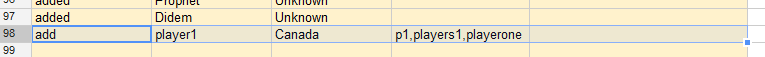
\includegraphics[width=0.80\columnwidth]{add_player}
\label{fig:add_player}
}
\subfigure[Add Player Error]{
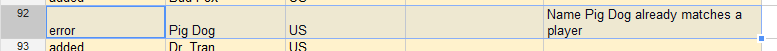
\includegraphics[width=0.80\columnwidth]{add_player_error}
\label{fig:add_player_error}
}
\caption{Adding a Player}
\end{figure}

If the status remains on add, then the player has not yet been added but will be added once the spreadsheet has been updated via the script. Once the player has actually been added to the system, the status will change from \texttt{add} to \texttt{added}. If there was some kind of error during adding, such as a duplicate player, then the status will be changed to \texttt{error} as seen in \figurename\ \ref{fig:add_player_error}.

\subsection{Adding Records}
The most involved process is adding a record. Adding a record is available through the \texttt{Add Record1} worksheet for Left 4 Dead 1 records and the \texttt{add Record 2} worksheet for Left 4 Dead 2 records. When adding records, the names used must already exist in the system. Otherwise, errors will appear during the script update process. The following fields must be filled out to add a record:
\begin{description}
\item[status] Set status to \texttt{add}.
\item[date] Put the date that the game took place in the format year-month-day, e.g., \texttt{2012-03-21} for March 21, 2012.
\item[time] Put the time that the game lasted here. There are two possible formats.
	\begin{itemize}
	\item minutes:seconds.hundredths of a second, e.g., \texttt{38:29.73} for 38 minutes, 29 seconds, and 73 hundredths of a second or 730 milliseconds. The number of minutes can exceed 60.
	\item hours:minutes:seconds.hundredths of a second, e.g., \texttt{01:28:29.23} means 1 hour, 28 minutes, 29 seconds, 230 milliseconds.
	\end{itemize}
\item[map] The name of the map played. This name must be the same name listed in the \texttt{Maps} worksheet.
\item[players] The name of all the players that played the game separated by commas (no spaces). Each of the names written here must match either a name or alias in the \texttt{Players} worksheet.
\item[common] Number of common infected killed
\item[hunters] Number of hunters killed
\item[smokers] Number of smokers killed
\item[boomers] Number of boomers killed
\item[chargers] Number of chargers killed (Left 4 Dead 2 only)
\item[spitters] Number of spitters killed (Left 4 Dead 2 only)
\item[jockeys] Number of jockeys killed (Left 4 Dead 2 only)
\item[tanks] Number of tanks
\item[groups] Add either a game mode or a strategy here (explained in Section \ref{sec:groups}) that applied to this survival game. Do not add playergroups. If there are multiple groups applicable, separate them with commas (no spaces).
\end{description}

Once the record has been added to the list, the status will say \texttt{added} and the record will be considered for all of the statistics that apply including normal statistics, top 10 statistics, and group statistics. If there was an error due to incorrect values, the status will say \texttt{error} and a corresponding error message will show up in the \texttt{errors} column. An example of adding a record is shown in \figurename\ \ref{fig:add_record} and an example error message is shown in \figurename\ \ref{fig:add_record_error}.
\begin{figure}[htb!]
\centering
\subfigure[Adding a New Record]{
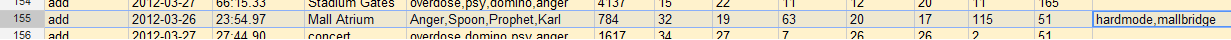
\includegraphics[width=\columnwidth]{add_record_example}
\label{fig:add_record}
}
\subfigure[Add Record Error]{
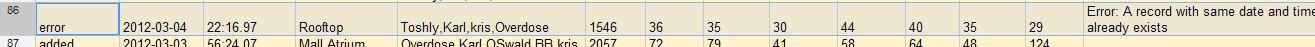
\includegraphics[width=\columnwidth]{add_record_error}
\label{fig:add_record_error}
}
\caption{Adding a Record}
\end{figure}

\section{Future Work}
A major future work addition will be to migrate the records into a proper database such as MySQL or SQLite. This was not done in the first place because of my lack of knowledge of databases. However, I might be willing to learn more about them and how to interface with them through Python as a hobby. I might also consider creating a graphical user interface for the script in the future. Other future work:
\begin{itemize}
\item Basic error checking has been added but more can be made for invalid inputs
\item Some basic functionality has been added for groups but creating and editing groups should be added.
\item More work on the documentation, specifically for spreadsheet maintainers and script developers.
\item The script is very slow and feels hacked together. Some major refactoring would be in order but I may never get around to doing this.
\end{itemize}
 
\bibliographystyle{IEEEtran}
\bibliography{./refs}

%\marginpar{\centering $\diamondtimes$}
\end{document}
